% Auto-generated by generated_analysis/summarize_project_plan_results.py
\subsection{Connection To The Original Project Plan}
The original project plan proposed a small-scale framework for testing whether videos preserve basic physical regularities over time. The present work keeps this aim but introduces controlled simulation as the main source of ground-truth dynamics. This change was made because early AI-generated videos were useful for pipeline validation but did not provide reliable labels for physical correctness.

The resulting benchmark directly supports the embedding-based temporal analysis proposed in the plan. Correct and wrong pendulum dynamics are compared through latent trajectory metrics, pairwise trajectory separation, and selected patch-level feature and attention visualisations. Collision and occlusion/object permanence remain natural extensions for the final version of the benchmark.

\begin{figure}[htbp]
\centering
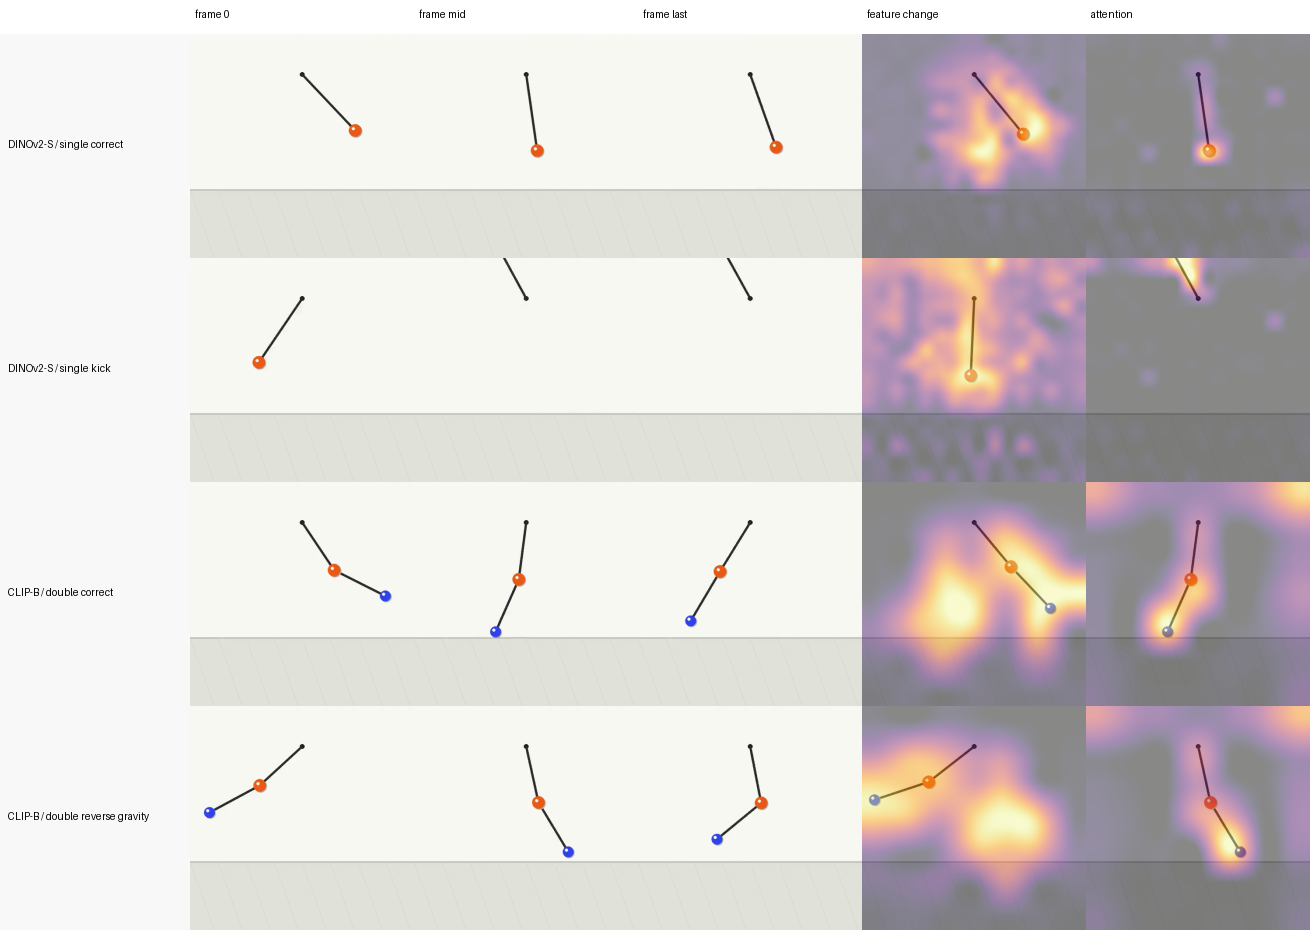
\includegraphics[width=\textwidth]{generated/simulated_pendulum/qualitative/qualitative_case_montage.png}
\caption{Selected qualitative case studies. Each row shows sampled frames, a patch feature-change map, and an attention overlay when available.}
\label{fig:qualitative-case-montage}
\end{figure}